% cone20-simple.tex

\section{Mach 1.5 flow over a 20$^o$ cone -- Simple boundaries}
\label{cone20-simple-sec}
%
This is an abstract example in that it models the flow of an ideal inviscid gas
over a sharp-nosed cone with 20 degree half angle and zero angle of incidence.
The resulting flow, in the steady-state limit, should have a single, 
straight (conical) shock that can be checked against classical gas-dynamic theory.
It is also a small (in both memory and run time) example 
that is useful for checking that the simulation and
plotting programs have been built or installed correctly.

\medskip
Assuming that you have the program executable files built and
accessible on your system's search \texttt{PATH}, 
try the following commands:\\
%
\topbar\\
\texttt{\$ cd $\sim$/cfcfd3/examples/eilmer3/2D/cone20-simple/}\\
\texttt{\$ ./cone20\_run.sh}\\
\bottombar\\
%
and, within a minute or so, you should end up with a number of files
with various solution data plotted.
The grid and initial solution are created and the time-evolution of the
flow field is computed for 5\,ms (with 1105 time steps being required).
The commands invoke the shell scripts displayed in 
subsection~\ref{cone20-sh-files}.
%

\begin{figure}[htbp]
\begin{center}
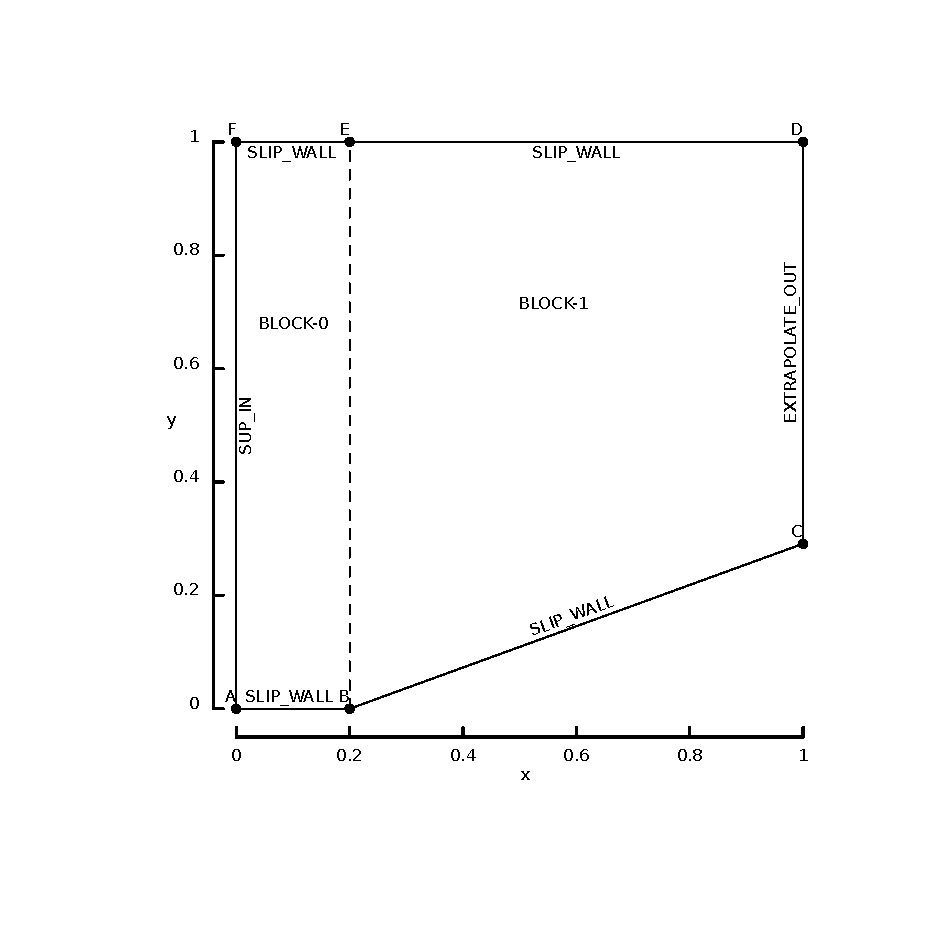
\includegraphics[width=10cm, viewport=76 78 389 398]{../2D/cone20-simple/cone20_svg.pdf}
\end{center}
\caption{Schematic diagram of the geometry for a cone 
         with 20 degree half-angle.
	 This PDF figure was generated from the SVG file with some edits 
	 to move the boundary labels to nicer positions.}
\label{cone20-geometry-fig}
\end{figure}

\medskip
The free-stream conditions ($p_{\infty} = 95.84$\,kPa, $T_{\infty} = 1103$\,K
and $u_{\infty} = 1000$\,m/s) are related to the shock-over-ramp test problem
in the original ICASE Report\,\cite{jacobs_91d} and are set to give a 
Mach number of 1.5.
From Chart 5 in Ref.\,\cite{ames_53}, the expected steady-state shock wave
angle is 49$^o$ and, from Chart 6, the pressure coefficient is
$$
\frac{p_{cone-surface} - p_{\infty}}{q_{\infty}} \approx 0.387
$$
and the dynamic pressure for the specified free stream is
$q_{\infty} = \frac{1}{2} \rho_{\infty} u_{\infty}^2 \approx 151.38$\,kPa.
Figure~\ref{cone20-axial-force-fig} shows the pressure coefficient 
estimated as
$$
C_p = \frac{f_x - p_{\infty} A}{q_{\infty} A}
$$
from the simulated axial force, $f_x$, written into the simulation log file
and frontal area of the cone, $A$.

\begin{figure}[htbp]
\begin{center}
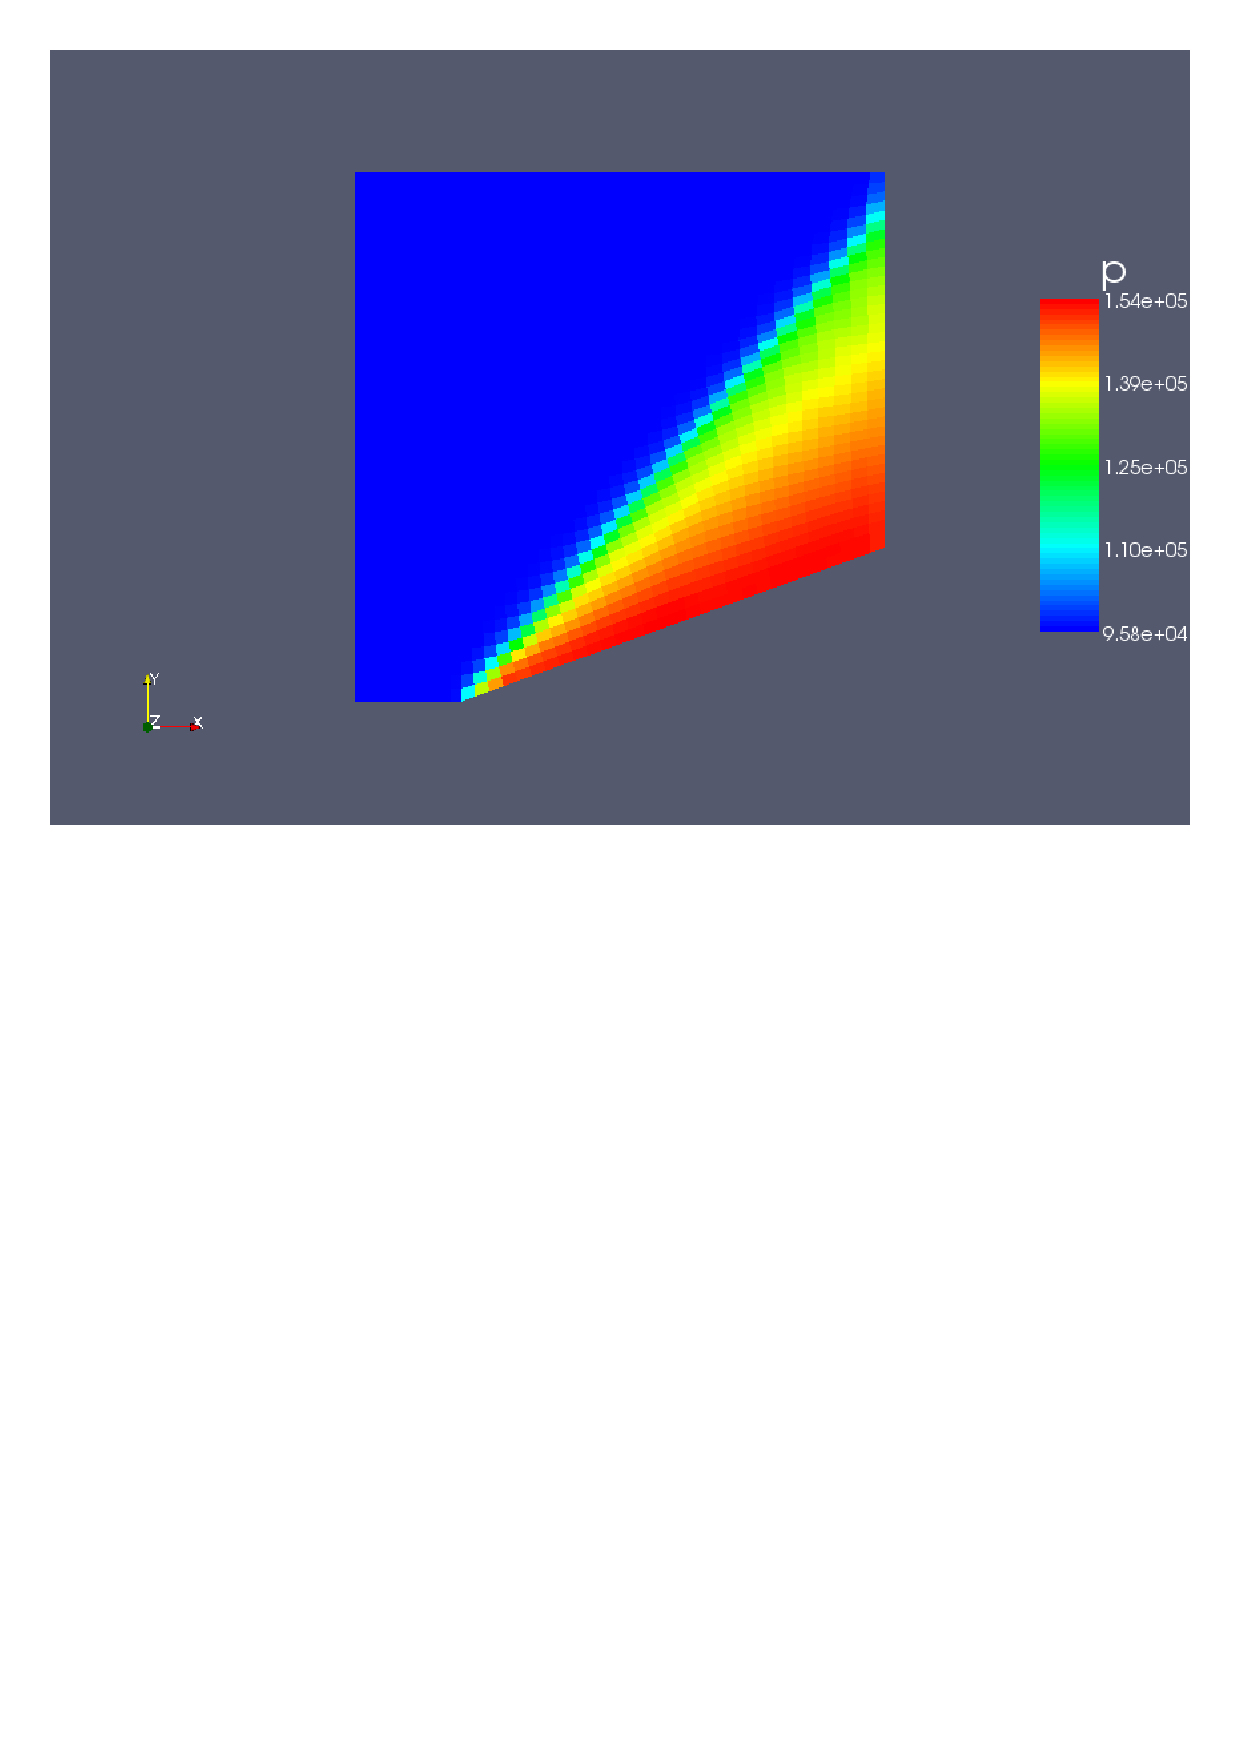
\includegraphics[width=0.8\textwidth, viewport=24 447 571 819]{../2D/cone20-simple/cone20_p.pdf}
\end{center}
\caption{Pressure data for flow over a cone with 20 degree half-angle.
         The shock profile is not yet straight and the pressure field
         near the cone surface is not conically symmetric, although it
	 would become more so if we continued the simulation.}
\label{cone20-pressure-fig}
\end{figure}

\begin{figure}[htbp]
\begin{center}
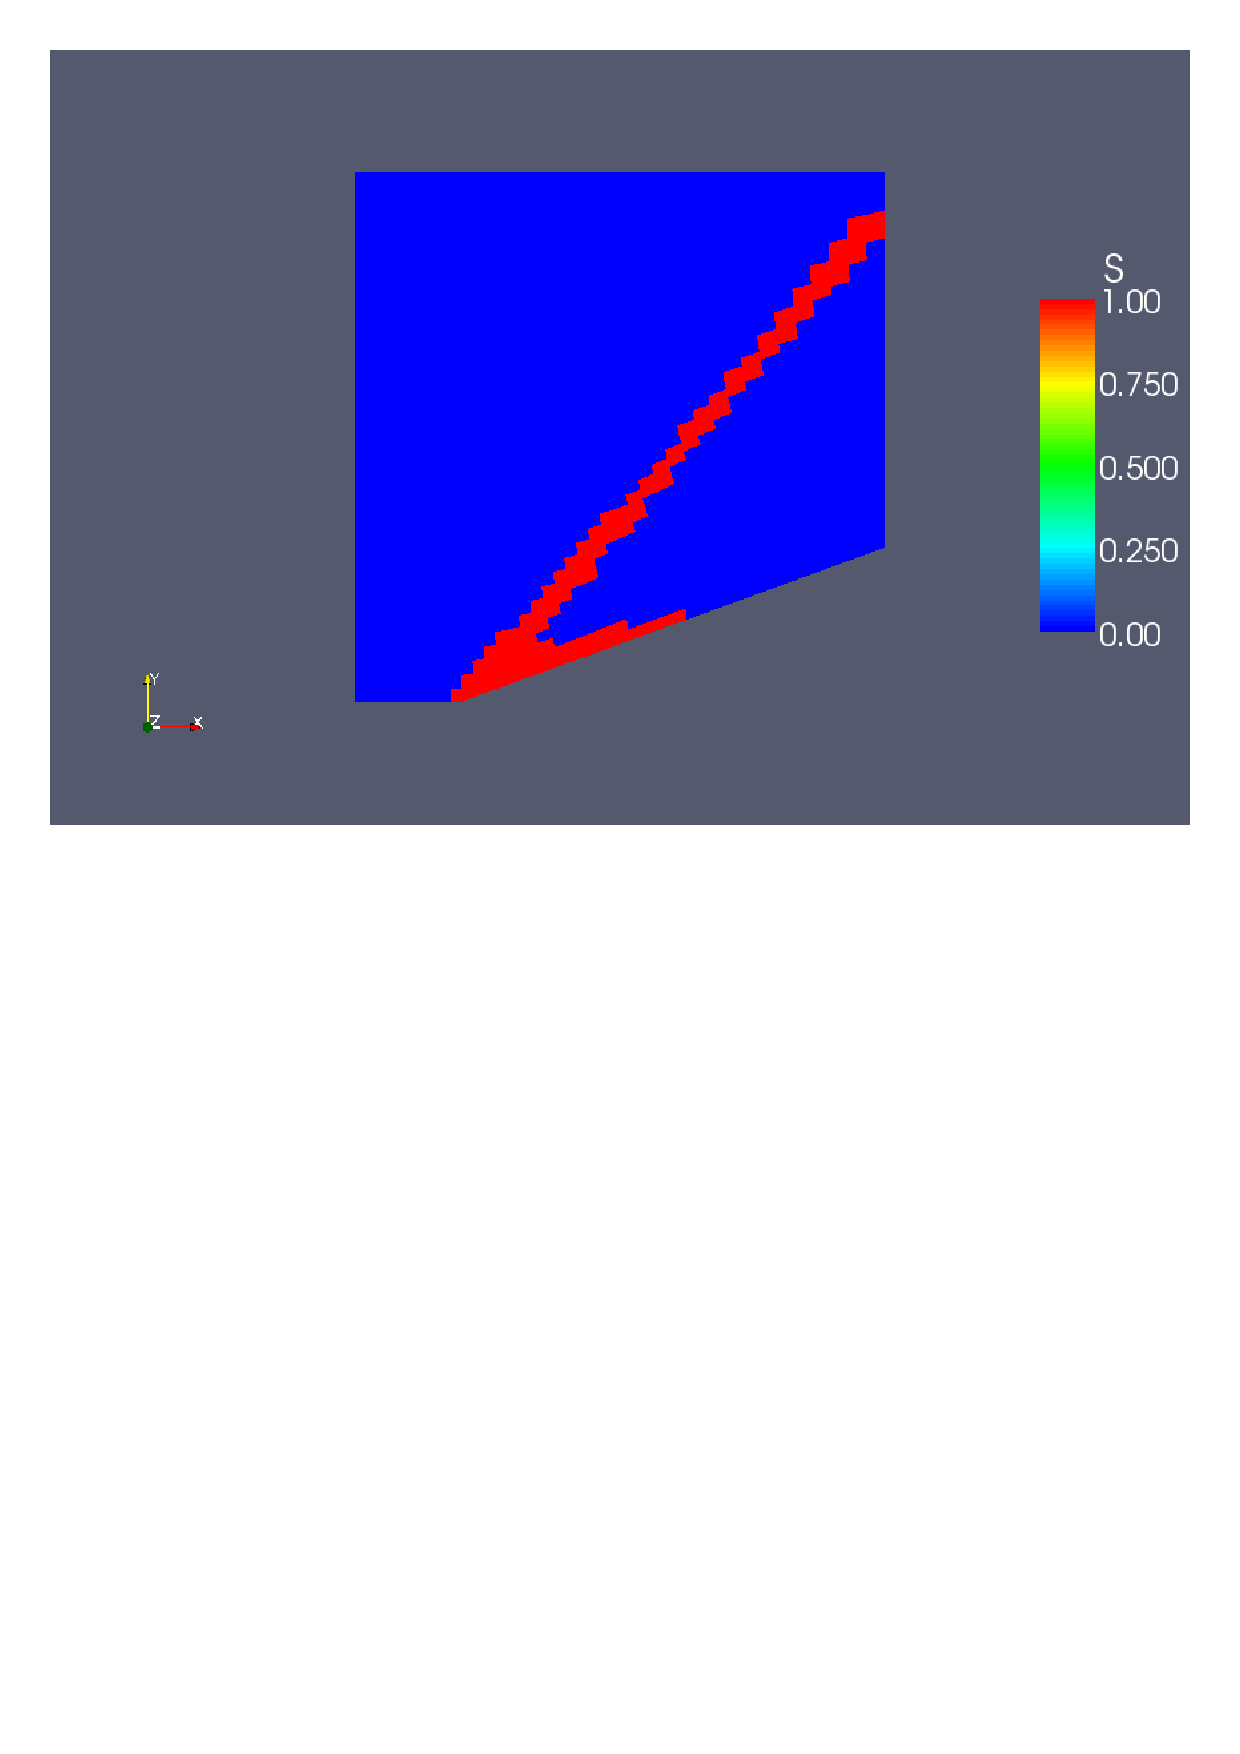
\includegraphics[width=0.8\textwidth, viewport=24 447 571 819]{../2D/cone20-simple/cone20_S.pdf}
\end{center}
\caption{Shock-sensor data for flow over a cone with 20 degree half-angle.
         For the \texttt{adaptive} flux calculator, 
	 this sensor indicates the regions
	 of the flow where the more dissipative scheme should be used.}
\label{cone20-shock-sensor-fig}
\end{figure}

\begin{figure}[htbp]
\begin{center}
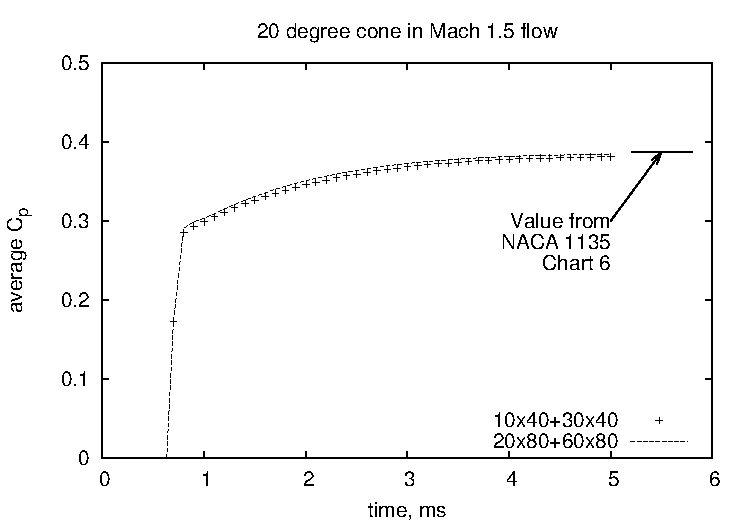
\includegraphics[width=10cm, viewport=52 49 401 294]{../2D/cone20-simple/cone20_cp.pdf}
\end{center}
\caption{Evolution of the axial (drag) force
         for flow over a cone with 20 degree half-angle
	 for two mesh resolutions.}
\label{cone20-axial-force-fig}
\end{figure}

\newpage

\subsection{Input script (.py)}\index{boundary conditions!set\_BC!example of use}
\topbar
\lstinputlisting[language={}]{../2D/cone20-simple/cone20.py}
\bottombar


\subsection{Shell scripts}
\label{cone20-sh-files}
\topbar
\lstinputlisting[language={}]{../2D/cone20-simple/cone20_run.sh}
\bottombar

\subsection{More specialized postprocessing}
\label{cone20-post-processing}
%
Beyond the usual slice-and-dice type of postprocessing, it may be useful to do
specialized calculations on the flow data.
Here, for example, the shock is expected to be straight and at an angle of 49.7$^o$ with
respect to the free-stream direction (Chart 5 in Ref.\,\cite{ames_53}).
The \texttt{estimate\_shock\_angle.py} script uses the Python code libraries 
that the \texttt{e3post.py} is built upon to pick up the data, 
locate the shock position along each strip of cells in the x-direction,
and then fit a straight line to the collected points.
Note that the points from the top right of the flow solution are omitted from the straight-line fit
because the top boundary has interfered with the flow.
The shock points and the fitted line are shown in Fig.\ref{cone20-shock-points-fig} 

\begin{figure}[htbp]
\begin{center}
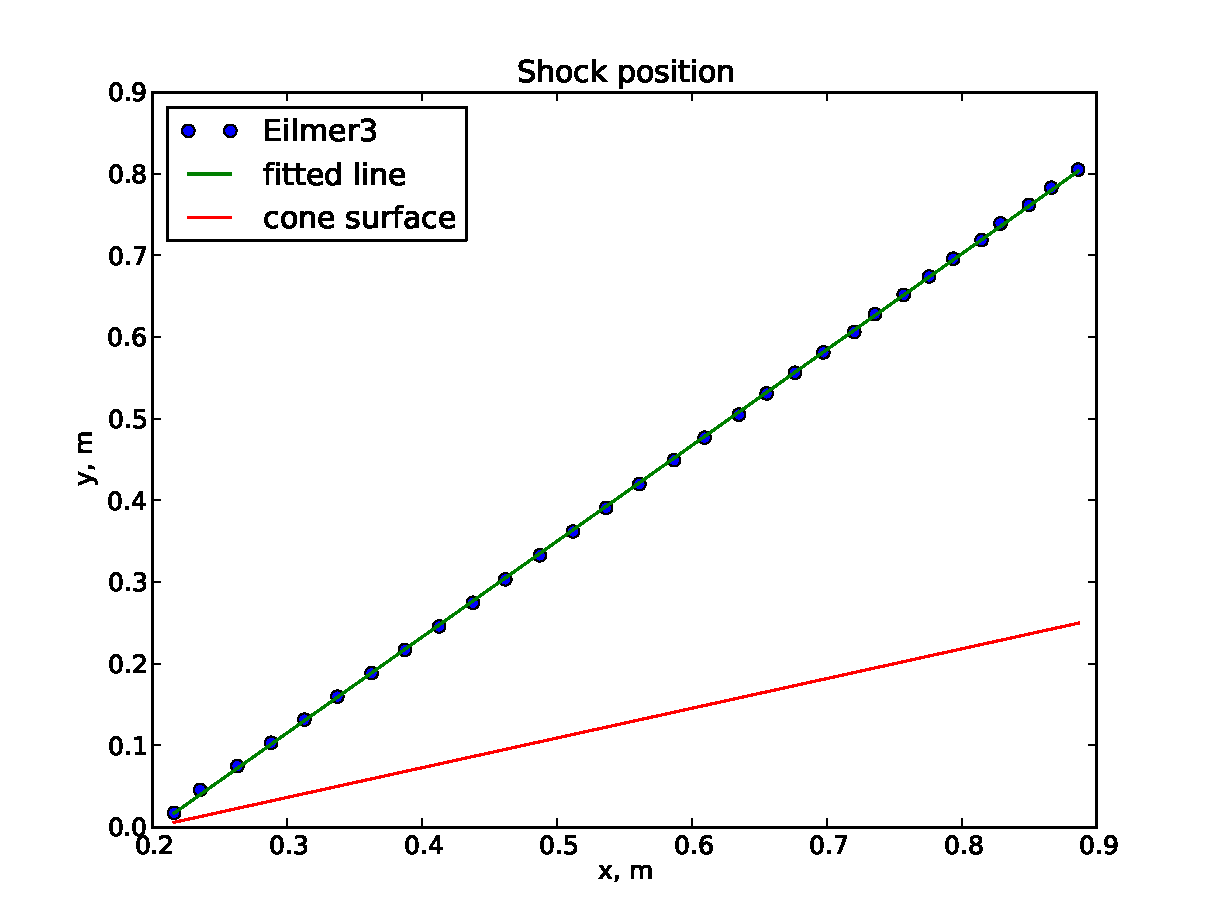
\includegraphics[width=10cm]{../2D/cone20-simple/shock-shape.pdf}
\end{center}
\caption{Shock shape for Mach 1.5 flow over the 20-degree cone.}
\label{cone20-shock-points-fig}
\end{figure}

The script below uses the data reading and storage capability provided by 
the class \texttt{StructuredGridFlow}, which is imported from \texttt{e3\_flow.py}.
Given a file containing the flow data for a block of cells, this class has a \texttt{read} 
method that picks up the data.
The flow and position data is stored in a dictionary, with one multidimensional numpy array 
for each variable.
Access to the pressure in cell \texttt{i,j,k} of block \texttt{ib,jb} is achieved by
putting these indices together as \texttt{blockData[ib][jb].data['p'][i,j,k]}.
The core of the data handling is in the function \texttt{locate\_shock\_front()}
in the middle of the script.

\noindent
\topbar
\lstinputlisting[language={}]{../2D/cone20-simple/estimate_shock_angle.py}
\bottombar

\subsection{Notes}
\begin{itemize}
\item Remember that long-format command-line options start with two dashes.
      For example \texttt{--job=cone20}.
      These double dashes are a little hard to distinguish in the shell
      scripts.

\item Run time is approximately 79 seconds for 1126 steps on a computer with 
      an Intel Dual Pentium E2160, 1.6\,GHz processor.
      As of September 2008, we have much optimisation to do.
      Of course, the shared-memory code does not make use of the second processor,
      however, there is an MPI version of the code that can.

\item This cone20.py file really has full access to the Python interpreter
      on your system.  Later examples will show how to use Python to write
      data files from within the input script.  Be careful.

\item Python is a dynamic language.
      It is easy to bind names to new objects within your script.
      Be careful that you do not rebind essential names that will be
      later used by the \texttt{e3prep.py} program.
      Where this might happen in a non-obvious way is in the importing
      of foreign modules (to do something interesting in your script)
      with the command ``from \textit{module-name} import *''.

\item Awk script for extracting x-force data from the simulation log file.
      New users might like to use an equivalent program written in Python.
      \lstinputlisting[language={}]{../2D/cone20-simple/cp.awk}\index{xforce\_list!example of use}

\item The script \texttt{cone20\_run\_mpi.sh} is available for running the simulation
  with the parallel version of the code on a machine with LAM-MPI installed.
  This script is essentially the same as shown for the shared-memory simulation
  with the MPI simulation being started with the commands:\index{e3mpi.exe!example of use}
\begin{verbatim}
mpirun -np 2 e3mpi.exe -f cone20 --run
\end{verbatim}
  The only other modification required is to look for the surface-force data in the
  log file \texttt{e3mpi.0001.log} rather than \texttt{e3shared.log}.

\item It turned out to be handy 
  (while trying to debug one of those nasty memory segmentation violations) 
  to be able to run the debug version of the MPI code within the valgrind 
  instrumentation and profiling environment with the commands:
\begin{verbatim}
$ cd ~/work/eilmer3/2D/cone20-simple/
$ script xxxx
$ mpirun -np 2 valgrind --tool=memcheck e3mpi.exe -f cone20 --run
$ exit
\end{verbatim}
  The \texttt{script} and \texttt{exit} start and stop recording of all of the console output
  to the file \texttt{xxxx}.
  If you have a few errors, valgrind output can be verbose.

\end{itemize}
